\subsection{Translational Controller Simulation}
The translational position and velocity controllers have been simulated with the non-linear model and the results are shown in the graphs below. \fxnote{Check the numbers in the whole section}

In order to test the translational velocity controller, as step reference has been given to the controller. The response is shown in figure \autoref{fig:TransVelocityControl}.
\begin{figure}[H]
	\centering
	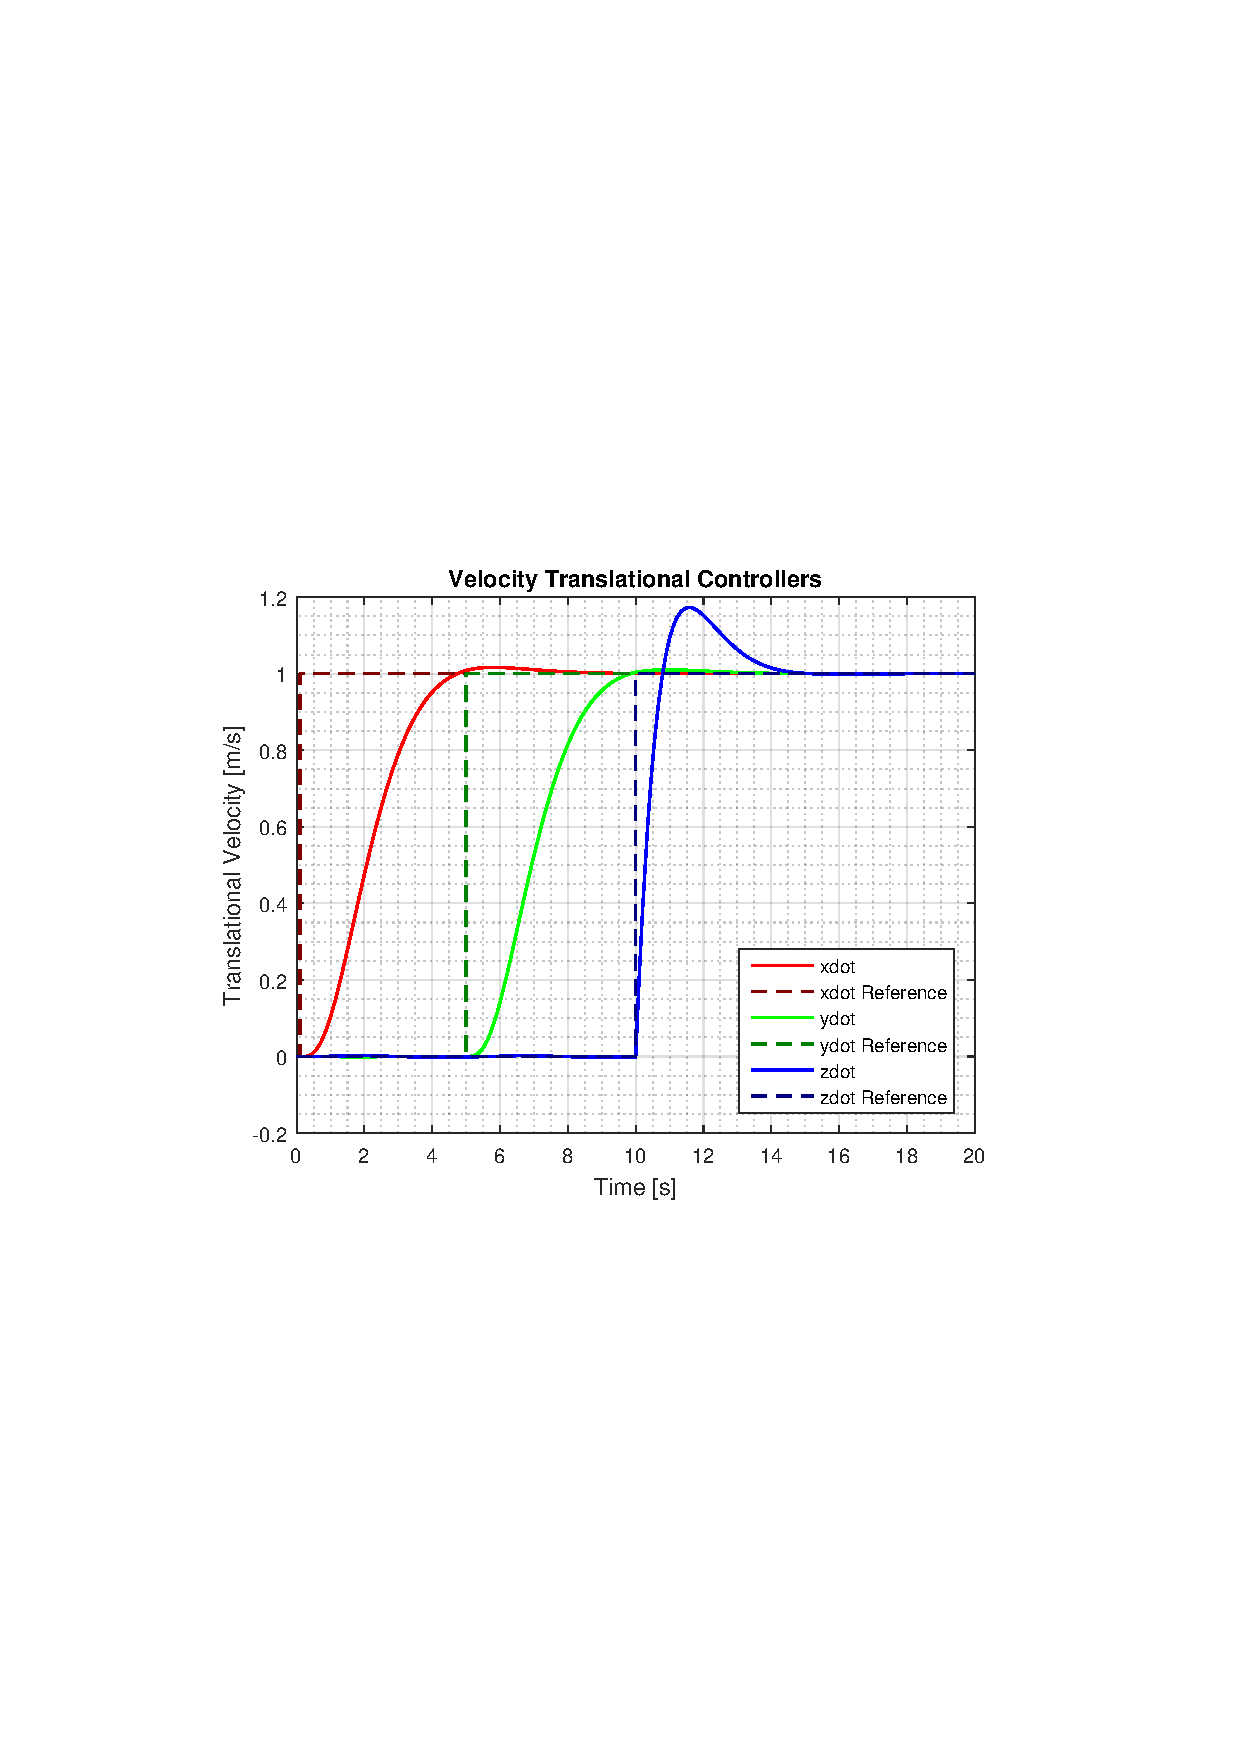
\includegraphics[scale=0.65]{figures/simVelocityController}
	\caption{Step response of the translational velocity controller along the three inertial axes direction.}
	\label{fig:TransVelocityControl}
\end{figure}
It can be seen that the velocity reference is attained in all axes with no steady state error in less than two seconds for the x and y velocity controller. The velocity  controller in z direction shows no steady state error either, but it shows an overshoot of less than 20 percent. This overshoot is acceptable as this controller is placed as the inner loop in the cascade translational controllers. The settling time for this controller is approximately 2.5 seconds.

The control output of the translational velocity controllers is shown in \autoref{fig:TransVelocityControlAngles}. These outputs are the references for the inner attitude controller, which has also been simulated to evaluate its reference tracking capabilities when acting in an inner loop.
\begin{figure}[H]
	\centering
	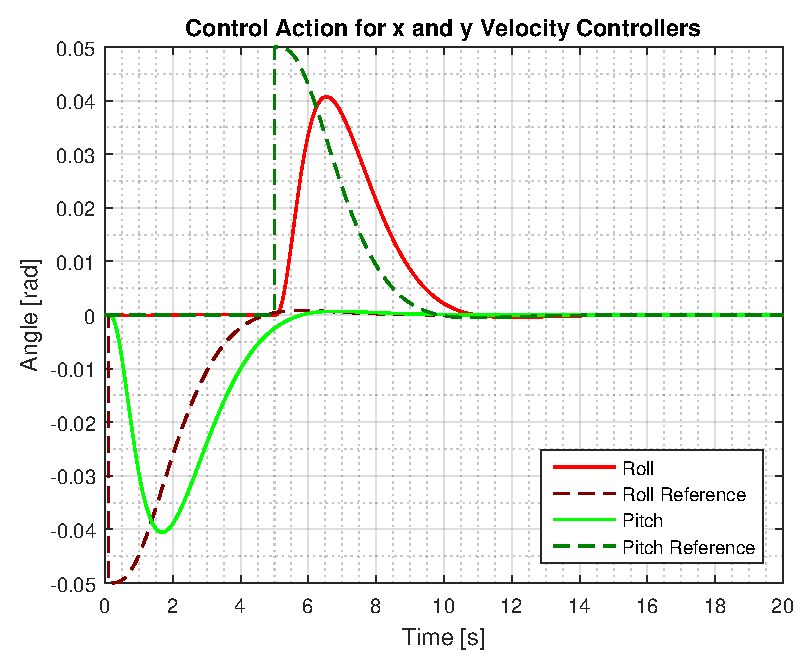
\includegraphics[scale=0.65]{figures/simVelocityControllerAngles}
	\caption{Attitude controller performance when the reference is set by the translational x and y velocity controller}
	\label{fig:TransVelocityControlAngles}
\end{figure}
It is worth mentioning the steady state error of the attitude controller when tracking a non-constant reference. This is due to the integral control added in the state feedback, as this assumes that a constant reference is applied to the controller. This is not true in the system at hand, but the fact of the attitude controller being in an inner loop makes this error not relevant for the final performance of the translational controllers. 

The sum of motor rotational speeds required by the z controller is shown in \autoref{fig:TransVelocityControlsum}. As expected the equilibrium rotational speeds are used until the velocity along the z direction is to be changed, at 10 seconds.
\begin{figure}[H]
	\centering
	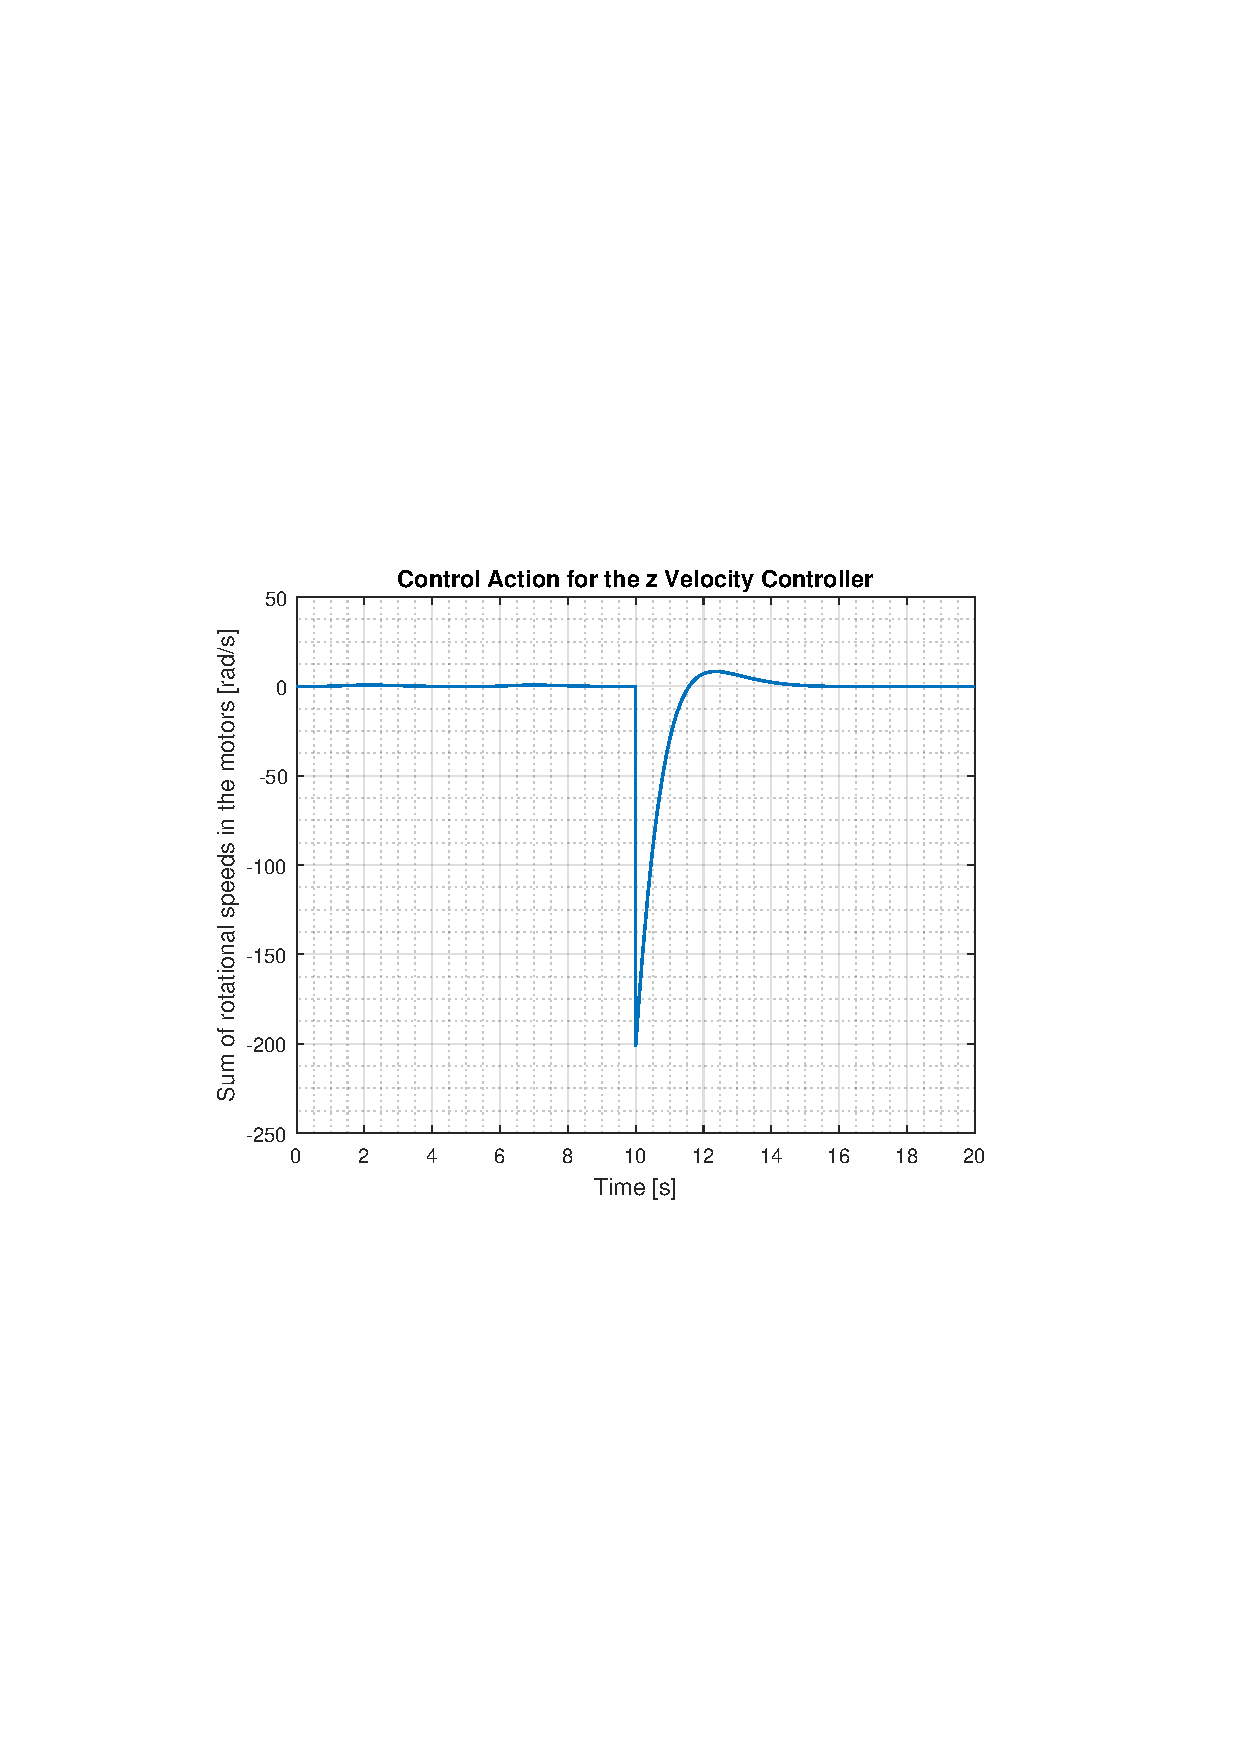
\includegraphics[scale=0.65]{figures/simVelocityControllerSum}
	\caption{Sum of motor rotational speeds required by the z translational velocity controller.}
	\label{fig:TransVelocityControlsum}
\end{figure}

The translational position controller response is shown in \autoref{fig:TranslationalControl}.
\begin{figure}[H]
	\centering
	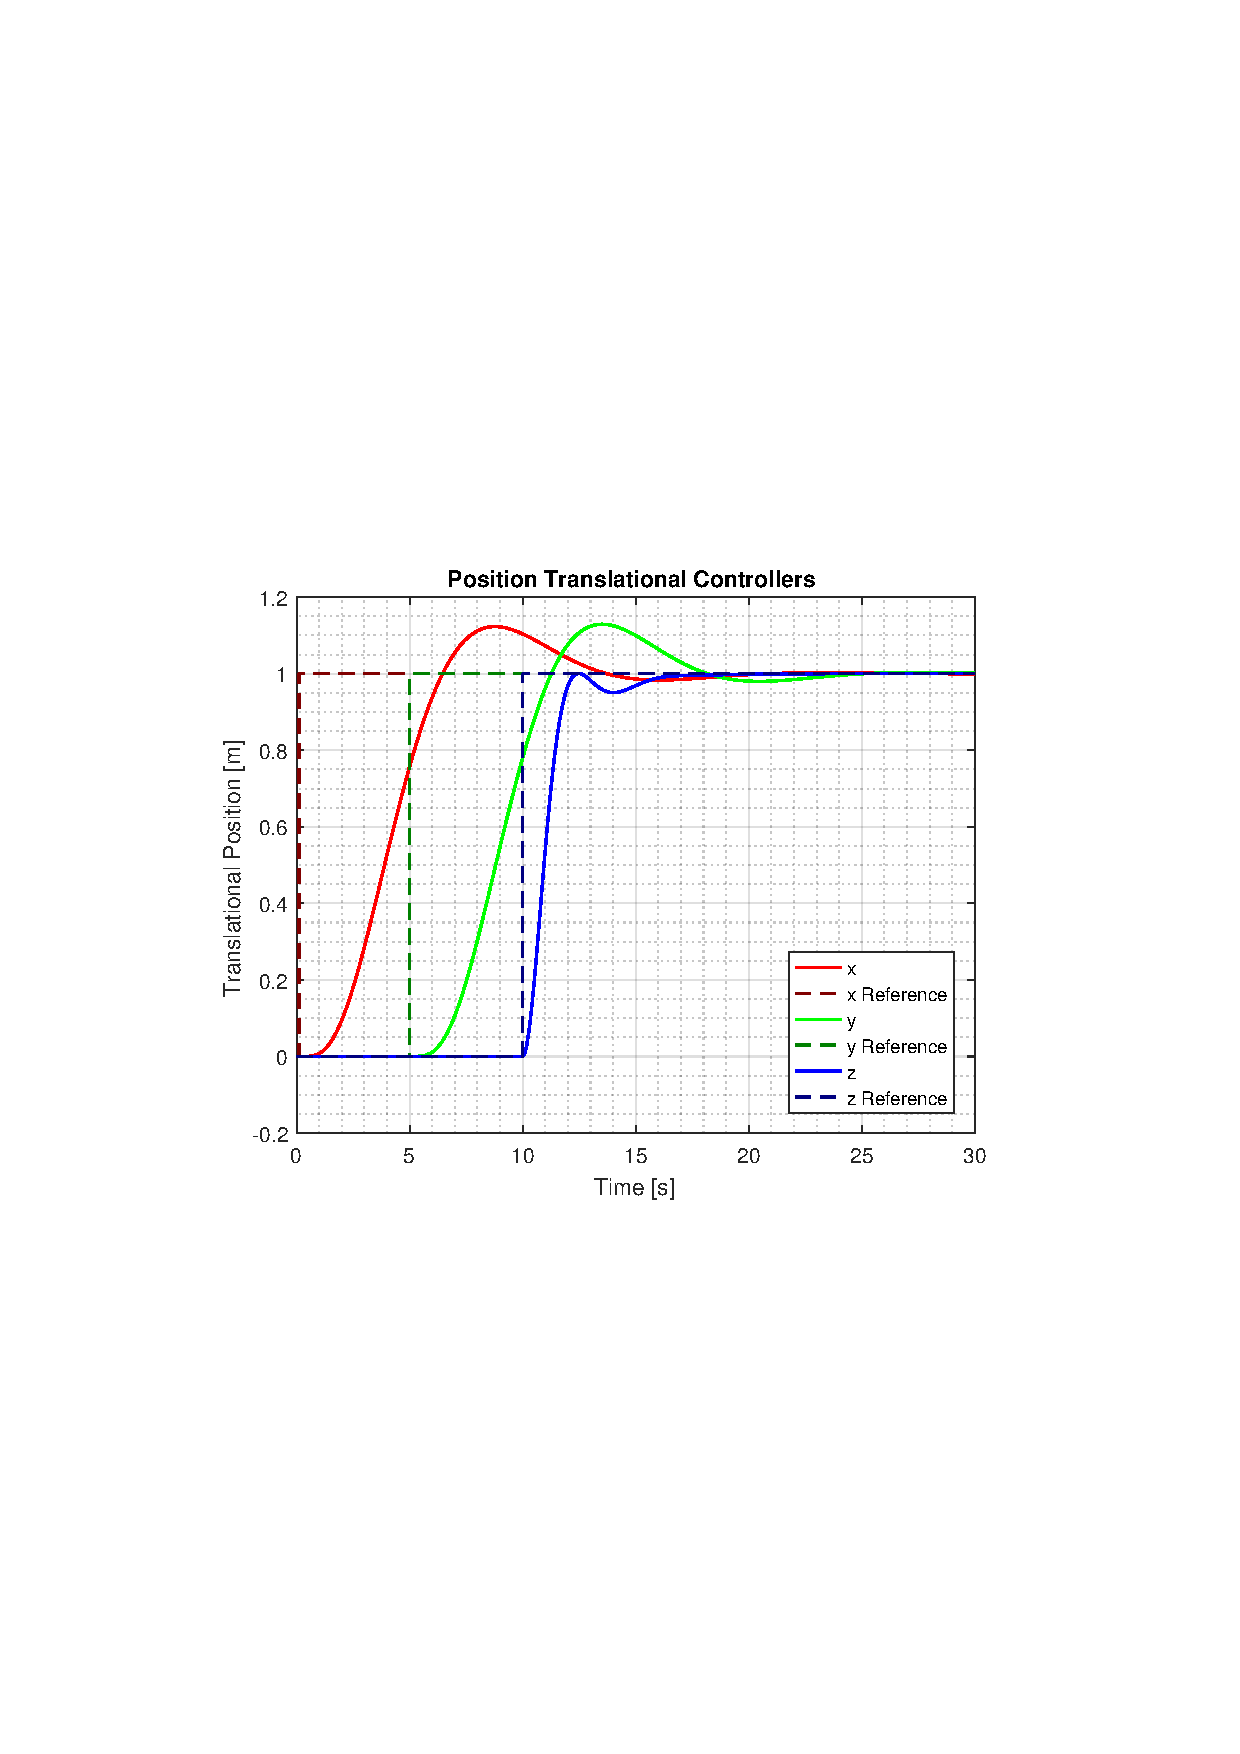
\includegraphics[scale=0.65]{figures/simTranslationalControl}
	\caption{Step response of the translational position controller along the three inertial axes direction.}
	\label{fig:TranslationalControl}
\end{figure}
All the position translational controllers perform well when tracking a reference as no steady state error is present in the simulations. The settling time of the x and y controllers is approximately 5 seconds and there is an overshoot of approximately 10 percent. his behavior is not represented by the transfer function and it is due to the inner velocity and attitude loops. 
The z controller has no overshoot, and the transient response seen on the curve corresponds to the inner velocity controller characteristics. This circumstance though, does not affect the final position and does not generate any overshoot. 

The control action is also evaluated through the references asked to the velocity controllers, see \autoref{fig:TranslationalControlOutput}, it can be seen that the inner loops perform well when tracking the given references.
\begin{figure}[H]
	\centering
	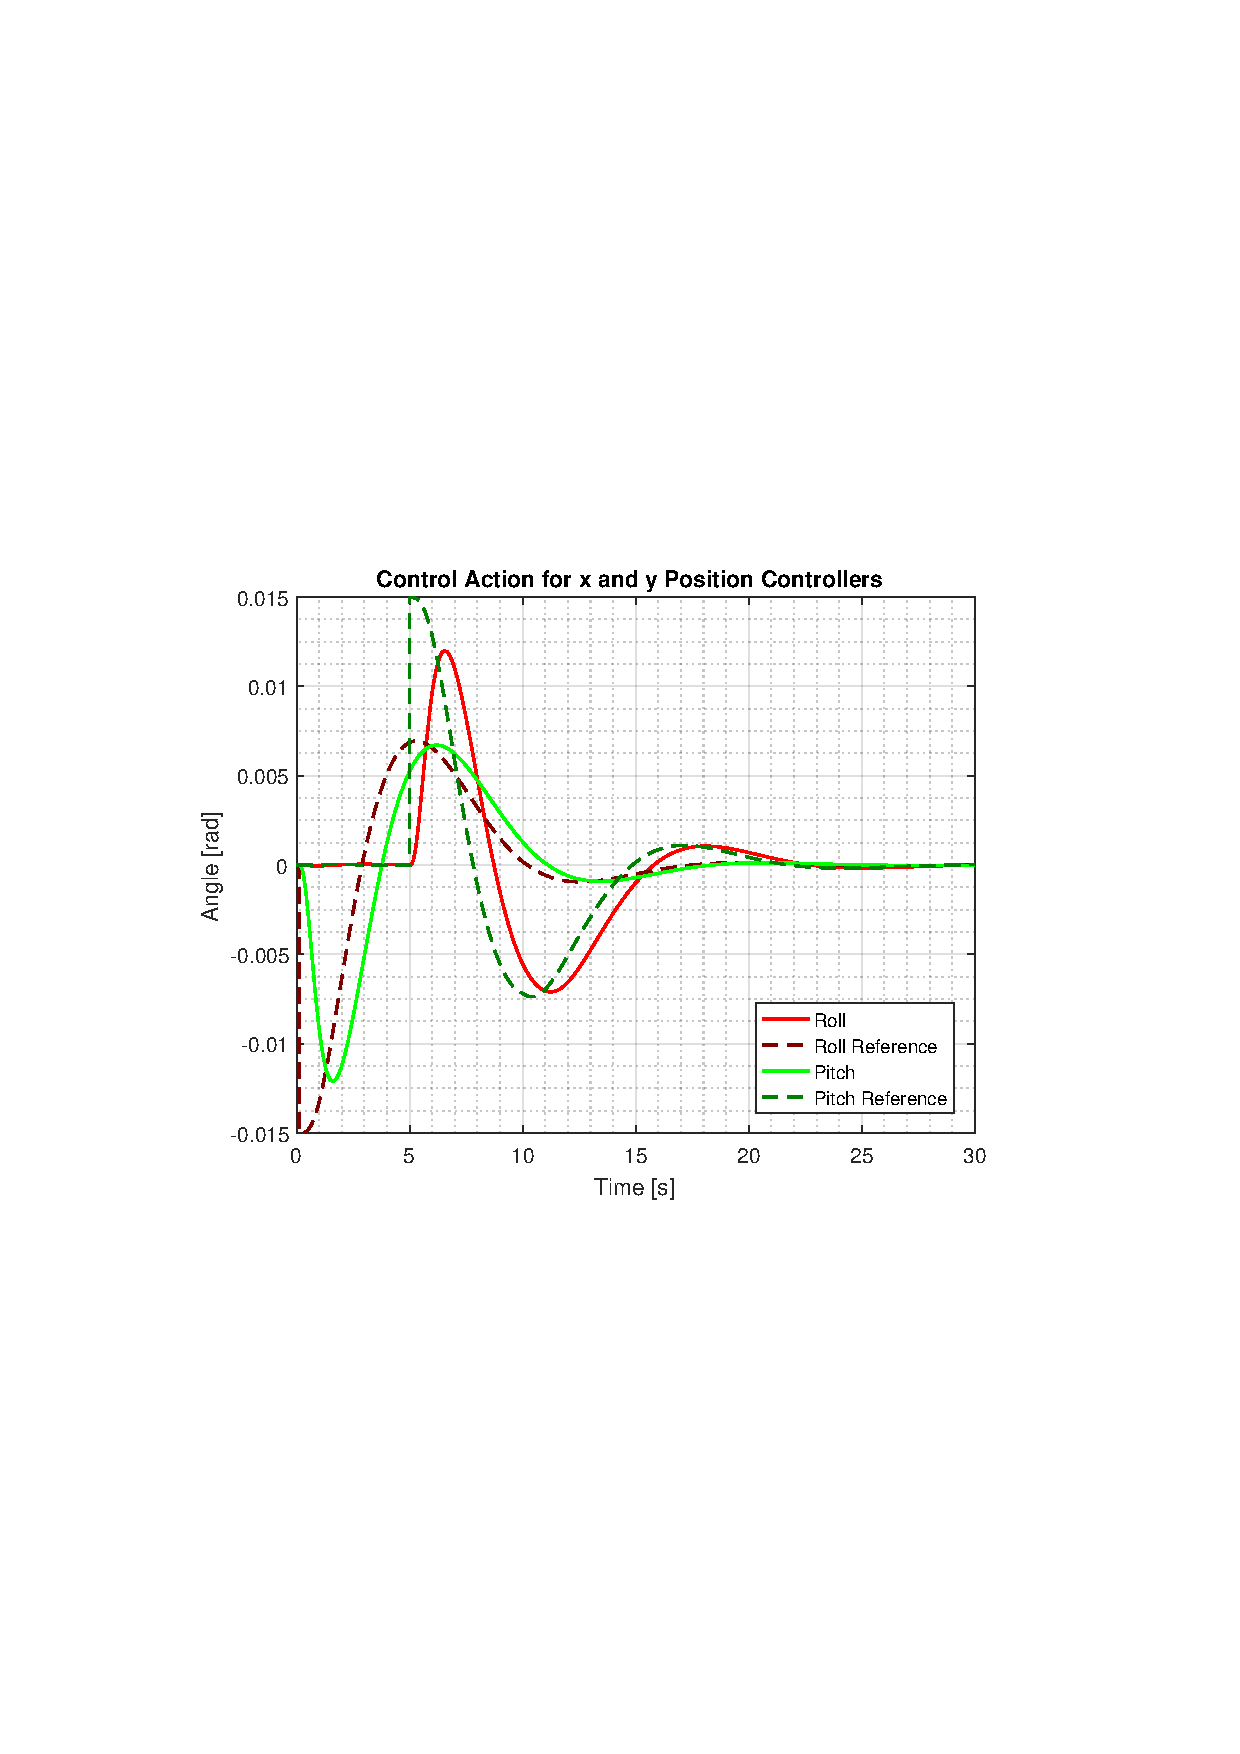
\includegraphics[scale=0.65]{figures/simTranslationalXYOutput}
	\caption{Attitude controller performance when the reference is set by the translational x and y velocity controller.\fxnote{Change figure}}
	\label{fig:TranslationalControlXYOutput}
\end{figure}
